%%%%%%%%%%%%%%%%%%%%%%%%%%%%%%%%%%%%%%%%%
% Stylish Curriculum Vitae
% LaTeX Template
% Version 1.0 (18/7/12)
%
% This template has been downloaded from:
% http://www.LaTeXTemplates.com
%
% Original author:
% Stefano (http://stefano.italians.nl/)
%
% IMPORTANT: THIS TEMPLATE NEEDS TO BE COMPILED WITH XeLaTeX
%
% License:
% CC BY-NC-SA 3.0 (http://creativecommons.org/licenses/by-nc-sa/3.0/)
%
% The main font used in this template, Adobe Garamond Pro, does not 
% come with Windows by default. You will need to download it in
% order to get an output as in the preview PDF. Otherwise, change this 
% font to one that does come with Windows or comment out the font line 
% to use the default LaTeX font.
%
%%%%%%%%%%%%%%%%%%%%%%%%%%%%%%%%%%%%%%%%%

\documentclass[a4paper, oneside, final]{scrartcl} % Paper options using the scrartcl class

\usepackage{scrpage2} % Provides headers and footers configuration
\usepackage{titlesec} % Allows creating custom \section's
\usepackage{marvosym} % Allows the use of symbols
\usepackage{tabularx,colortbl} % Advanced table configurations
\usepackage{fontspec} % Allows font customization
\usepackage{hyperref}
\usepackage{pbox}
\usepackage{ragged2e}

\defaultfontfeatures{Mapping=tex-text}
\setmainfont{EB Garamond} % Main document font

\titleformat{\section}{\large\scshape\raggedright}{}{0em}{}[\titlerule] % Section formatting

\pagestyle{scrheadings} % Print the headers and footers on all pages

\addtolength{\voffset}{-0.5in} % Adjust the vertical offset - less whitespace at the top of the page
\addtolength{\textheight}{3cm} % Adjust the text height - less whitespace at the bottom of the page

\newcommand{\gray}{\rowcolor[gray]{.90}} % Custom highlighting for the work experience and education sections

%----------------------------------------------------------------------------------------
% FOOTER SECTION
%----------------------------------------------------------------------------------------

\renewcommand{\headfont}{\normalfont\rmfamily\scshape} % Font settings for footer

\cofoot{
\addfontfeature{LetterSpace=20.0}\fontsize{12.5}{17}\selectfont % Letter spacing and font size

\href{https://fr.linkedin.com/in/oscar-laurent-52878215}{LinkedIn} {\large\textperiodcentered} 
\href{https://github.com/olaure/}{GitHub}
}

%----------------------------------------------------------------------------------------

\begin{document}

\begin{center} % Center everything in the document

%----------------------------------------------------------------------------------------
% HEADER SECTION
%----------------------------------------------------------------------------------------

\begin{tabularx}{\textwidth}{
	@{} >{\addfontfeature{LetterSpace=20.0}\fontsize{26}{26}\selectfont \scshape}l
	@{\hspace{3.7cm}} r 
	@{\hspace{0.5cm}} r
}
 \pbox{4cm}
 {
	 \href{https://fr.linkedin.com/in/oscar-laurent-52878215}{Oscar  
	 Laurent}\\
	 {\addfontfeature{LetterSpace=10.0}\fontsize{10}{10}\selectfont
	 D\'eveloppeur \  junior
	 }
  } &
 \pbox{5cm}{\RaggedLeft%\raggedright
  \href{http://www.openstreetmap.org/\#map=19/48.87250/2.30862}{8 rue d'Artois, Paris} \\ % Your mailing address
  osc.laurent@gmail.com \\
  \href{tel:0607109236}{06 07 10 92 36} % Your email address and phone number
 } &
 \raisebox{-.55\height}{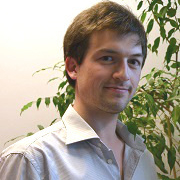
\includegraphics[width=3cm]{me.png}} % image baseline is at its bottom
\end{tabularx}

\vspace{1.5cm} % Extra whitespace after the large name at the top

%----------------------------------------------------------------------------------------
%	OBJECTIVE
%----------------------------------------------------------------------------------------

\section{Motivations}

 Je cherche un stage me permettant d'appliquer \`a une fin industrielle mes capacit\'es en acquisition et traitement de l'information au contact de professionnels de la S\'ecurit\'e.

\vspace{10pt}
%----------------------------------------------------------------------------------------
%	SKILLS
%----------------------------------------------------------------------------------------

\section{Comp\'etences}

\begin{tabular}{ @{} >{\bfseries}l @{\hspace{6ex}} l }
 Langages & C, bash, python 2.7, PHP, awk, fortran, JS, ruby \\
 Outils & vim, git, nmap \\
 Compétences & débug (gdb, lldb), optimisation, analyses statistiques \\ 
 Environnements & Windows, UNIX
\end{tabular}

%----------------------------------------------------------------------------------------
%	EDUCATION
%----------------------------------------------------------------------------------------

\section{\'{E}ducation}

\begin{tabularx}{0.97\linewidth}{>{\raggedleft\scshape}p{2cm}X}
\gray Période & \textbf{Novembre 2015 --- Aujourd'hui}\\
\gray Titre & \textbf{Architecte en technologie numérique}\\
\gray \'Ecole & \textbf{\href{http://www.42.fr}{\'{E}cole 42}} \hfill Paris, France\\
& Apprentissage d'algorithmes d'optimisation (A*, pathfinding) \\
& Gestion de projet interdisciplinaire en partenariat avec l'\href{http://www.ifm-paris.com/}{IFM} (scraping, ruby)
% 
\end{tabularx}

\vspace{12pt}

\begin{tabularx}{0.97\linewidth}{>{\raggedleft\scshape}p{2cm}X}
\gray Période & \textbf{Septembre 2012 --- Juillet 2016}\\
\gray Titre & \textbf{Thèse de Science en physico-chimie des matériaux}\\
\gray Université & \textbf{\href{http://www.upmc.fr/}{Université Paris 6}} \hfill Paris, France\\
& Analyses statistiques (C et fortran) de modélisations moléculaires \\
& (structures \`a courte et moyenne portées) de syst\`emes vitreux
\end{tabularx}

\vspace{12pt}

\begin{tabularx}{0.97\linewidth}{>{\raggedleft\scshape}p{2cm}X}
\gray Période & \textbf{Septembre 2011 --- Juillet 2012}\\
\gray Titre & \textbf{Master de Science en Physique}\\
\gray Université & \textbf{\href{http://www.univ-paris-diderot.fr/}{Université Paris 7}} \hfill Paris, France\\
& Utilisation de python pour faire du tracking de points sur videos
\end{tabularx}

\vspace{12pt}


%----------------------------------------------------------------------------------------
%	WORK EXPERIENCE
%----------------------------------------------------------------------------------------

%\section{Work Experience}
%
%\begin{tabularx}{0.97\linewidth}{>{\raggedleft\scshape}p{2cm}X}
%\gray Period & \textbf{March 2012 --- Present}\\
%\gray Employer & \textbf{Layer BV} \hfill Amsterdam, The Netherlands\\
%\gray Job Title & \textbf{J2EE Analyst programmer}\\
%\gray Languages & \textbf{J2EE}\\
%    & Lorem ipsum dolor sit amet, consectetur adipiscing elit. Donec et auctor neque. Nullam ultricies sem sit amet magna tristique imperdiet. Cum sociis natoque penatibus et magnis dis parturient montes, nascetur ridiculus mus. Phasellus eget mollis nunc.
%\end{tabularx}



%----------------------------------------------------------------------------------------

\end{center}

\end{document}
